\documentclass[12pt, oneside,fullpage]{article}

\usepackage{amsmath}
\usepackage{amssymb}
\usepackage{graphicx}
\usepackage{hyperref}
\usepackage[margin=1in]{geometry}

\newcommand{\Lc}{$\mathcal{L}$}

\title{Monty Hall Problem}
\date{October 16\textsuperscript{th}, 2019}

\begin{document}
\maketitle

\noindent There are three cups, and under one cup is a coin.

\begin{figure}[ht]
	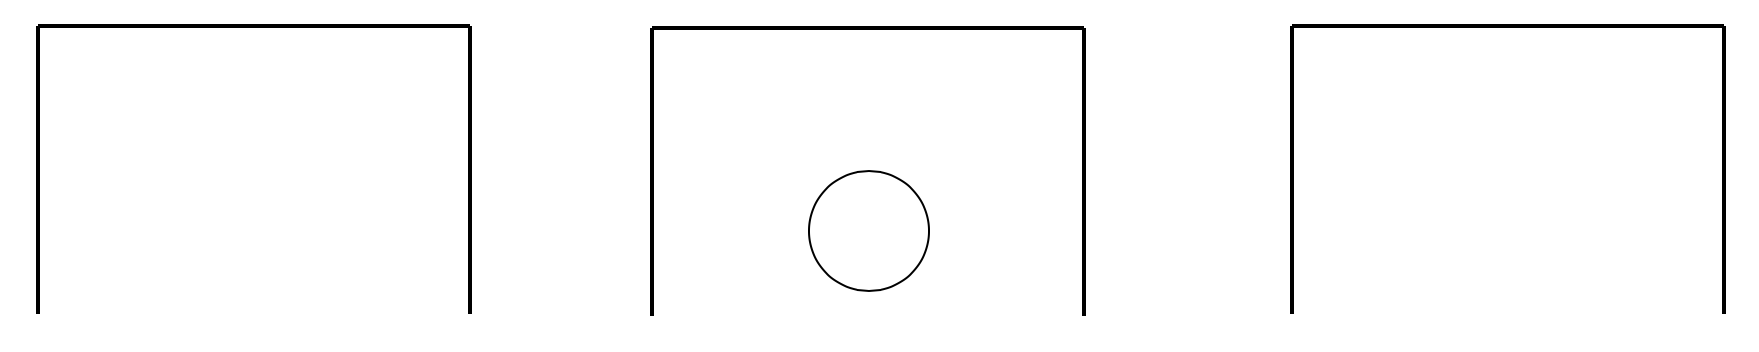
\includegraphics[width=5.0in, keepaspectratio]{Three_Cups.png}
\end{figure}


\noindent You pick one of the cups, and Monty Hall (MH) removes a cup without the coin. What is the probability that your cup has the coin?

\begin{figure}[ht]
	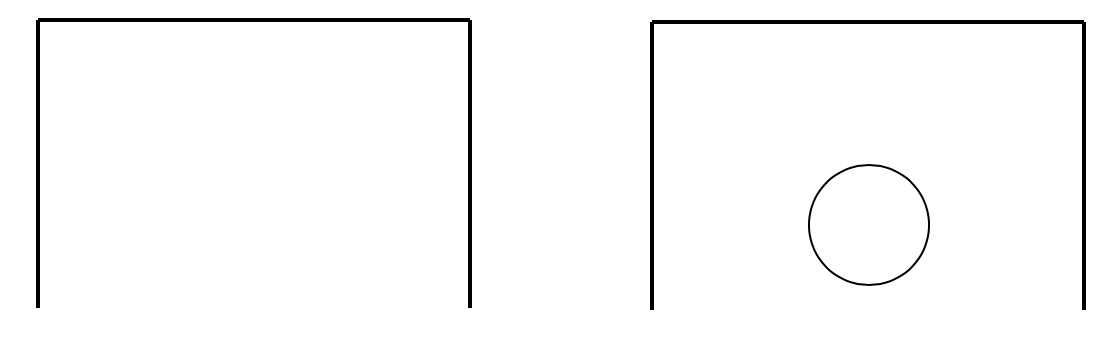
\includegraphics[width=3.2in, keepaspectratio]{Two_Cups.png}
\end{figure}


\noindent Start with P(X=x) = $\frac{1}{3}$, where x = cup 1, cup 2, cup 3. Now consider the scenario that the coin is under cup 1. One way of looking at this is that the probability of your cup having the coin has not changed, so it is still $1/3$ and thus the probability of the other cup having the coin is now $2/3$. Another way is as follows:

\bigskip

\noindent You pick x = cup 1 and it has the coin under it. MH removes cup 2 or 3.

P(X=1) $\cdot$ P(MH removes cup 1) +

P(X=1) $\cdot$ P(MH removes cup 2) + \indent  $\Rightarrow$ \indent  0 + $\frac{1}{3} \cdot \frac{1}{2} + \frac{1}{3} \cdot \frac{1}{2}$ $\Rightarrow \frac{1}{3}$

P(X=1) $\cdot$ P(MH removes cup 3)

\bigskip

\noindent You pick x = cup 2, but the coin is under is under cup 1!

P(X=2) $\cdot$ P(MH removes cup 1) +

P(X=2) $\cdot$ P(MH removes cup 2) + \indent  $\Rightarrow$ \indent 0 + 0 + $\frac{1}{3} \Rightarrow \frac{1}{3}$

P(X=2) $\cdot$ P(MH removes cup 3)

\bigskip

\noindent You pick x = cup 3, but the coin is still under cup 1!

P(X=3) $\cdot$ P(MH removes cup 1) +

P(X=3) $\cdot$ P(MH removes cup 2) + \indent  $\Rightarrow$ \indent  0 + $\frac{1}{3}$ + 0 $\Rightarrow \frac{1}{3}$

P(X=3) $\cdot$ P(MH removes cup 3)


\noindent Regardless of which cup you initially choose, you have a $\frac{1}{3}$ chance of winning, but a $\frac{2}{3}$ chance by switching cups.

This example works (ie, the probability is not $1/2$) because we have prior information about the position of the coin from the initial setup. Even though we did not know where it was, we still were able to learn where it wasn't.

\bigskip

\noindent Books on Bayesian stats

E.T Jaynes - a Bayesian manifesto

C Mackay: Interference - Practical guides to using Bayesian statistics

Gelman: Bayesian Data Analysis - Analysis techniques for various problems.

Ivezic \& others: Orange book: \url{https://www.amazon.com/Statistics-Mining-Machine-Learning-Astronomy/dp/0691151687} - The astrostatistics textbook

\bigskip

\begin{center}
	\LARGE{Markov Chain Monte Carlo}
\end{center}

The problem of MCMC is to sample a function well enough to draw a graph of errors. A simple way to do this is to sample at random or on a grid: if we generate enough random samples we will eventually find the maximum of the function. To make this concrete, for a likelihood, \Lc($x_{i}$), you have $x_{i}$ at random or $x_{i} = (\frac{i}{N}, \frac{i}{N}, \frac{i}{N})$

[Random sampling can be slow to fully map the \Lc, but if \Lc\ is pathological, random sampling may be the best you can do: other sampling methods are implicitly making assumptions about the smoothness of \Lc.]

We can do better by trying to find local peaks of the likelihood: we use our existing information about the state of the function to inform our random choices about where to go next.

\medskip

\noindent In practice, the easiest way is to use the emcee package in python: ``import emcee''

\medskip

\noindent How to check convergence of a chain:

Gelman-Rubin criterion: start multiple chains ($\sim4$), stop when the max(\Lc) of all chains is ``the same" (within 1\%).

The simplest MCMC algorithm is Metropolis-Hastings, about which more next time.

\end{document}
